

\tikzset{every picture/.style={line width=0.75pt}} %set default line width to 0.75pt        

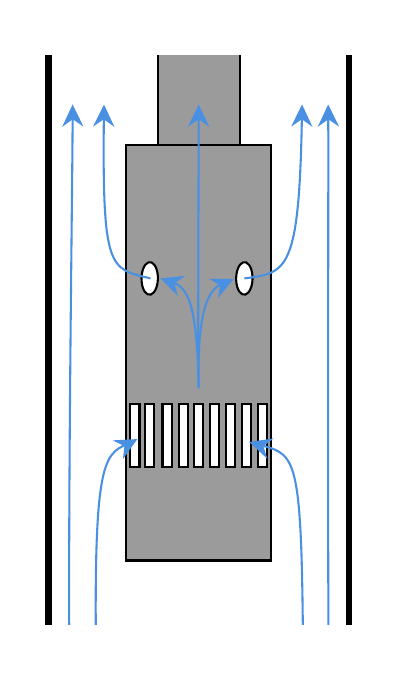
\begin{tikzpicture}[x=0.75pt,y=0.75pt,yscale=-1,xscale=1]
%uncomment if require: \path (0,406); %set diagram left start at 0, and has height of 406

%Shape: Rectangle [id:dp04480742808021354] 
\draw  [fill={rgb, 255:red, 155; green, 155; blue, 155 }  ,fill opacity=1 ] (312,64.14) -- (351.5,64.14) -- (351.5,114.5) -- (312,114.5) -- cycle ;
%Shape: Rectangle [id:dp3210354209072095] 
\draw  [line width=2.25]  (259.42,64.14) -- (404.08,64.14) -- (404.08,352) -- (259.42,352) -- cycle ;
%Shape: Rectangle [id:dp11917689807401133] 
\draw  [fill={rgb, 255:red, 155; green, 155; blue, 155 }  ,fill opacity=1 ] (296.75,114.5) -- (366.75,114.5) -- (366.75,314.5) -- (296.75,314.5) -- cycle ;
%Shape: Rectangle [id:dp22447305445205257] 
\draw  [fill={rgb, 255:red, 255; green, 255; blue, 255 }  ,fill opacity=1 ] (305.89,238.94) -- (310.33,238.94) -- (310.33,269.56) -- (305.89,269.56) -- cycle ;
%Shape: Rectangle [id:dp05751039520762724] 
\draw  [fill={rgb, 255:red, 255; green, 255; blue, 255 }  ,fill opacity=1 ] (314.33,238.94) -- (318.78,238.94) -- (318.78,269.56) -- (314.33,269.56) -- cycle ;
%Shape: Rectangle [id:dp6083474962263296] 
\draw  [fill={rgb, 255:red, 255; green, 255; blue, 255 }  ,fill opacity=1 ] (322.11,238.94) -- (326.56,238.94) -- (326.56,269.56) -- (322.11,269.56) -- cycle ;
%Shape: Rectangle [id:dp9699991258462393] 
\draw  [fill={rgb, 255:red, 255; green, 255; blue, 255 }  ,fill opacity=1 ] (329.53,238.94) -- (333.97,238.94) -- (333.97,269.56) -- (329.53,269.56) -- cycle ;
%Shape: Rectangle [id:dp5276274421172025] 
\draw  [fill={rgb, 255:red, 255; green, 255; blue, 255 }  ,fill opacity=1 ] (337,238.94) -- (341.44,238.94) -- (341.44,269.56) -- (337,269.56) -- cycle ;
%Shape: Rectangle [id:dp8686039431642814] 
\draw  [fill={rgb, 255:red, 255; green, 255; blue, 255 }  ,fill opacity=1 ] (344.78,238.94) -- (349.22,238.94) -- (349.22,269.56) -- (344.78,269.56) -- cycle ;
%Shape: Rectangle [id:dp024923249699371652] 
\draw  [fill={rgb, 255:red, 255; green, 255; blue, 255 }  ,fill opacity=1 ] (352.56,238.94) -- (357,238.94) -- (357,269.56) -- (352.56,269.56) -- cycle ;
%Shape: Rectangle [id:dp24614630976896423] 
\draw  [fill={rgb, 255:red, 255; green, 255; blue, 255 }  ,fill opacity=1 ] (360.11,238.94) -- (364.56,238.94) -- (364.56,269.56) -- (360.11,269.56) -- cycle ;
%Shape: Rectangle [id:dp4580617305504924] 
\draw  [fill={rgb, 255:red, 255; green, 255; blue, 255 }  ,fill opacity=1 ] (298.78,238.94) -- (303.22,238.94) -- (303.22,269.56) -- (298.78,269.56) -- cycle ;
%Curve Lines [id:da46150758694693694] 
\draw [color={rgb, 255:red, 74; green, 144; blue, 226 }  ,draw opacity=1 ]   (282.2,352) .. controls (281.45,261.49) and (287.15,263.11) .. (299.52,257.34) ;
\draw [shift={(302.2,256)}, rotate = 511.33] [fill={rgb, 255:red, 74; green, 144; blue, 226 }  ,fill opacity=1 ][line width=0.08]  [draw opacity=0] (10.72,-5.15) -- (0,0) -- (10.72,5.15) -- (7.12,0) -- cycle    ;
%Shape: Circle [id:dp04721201185159396] 
\draw  [fill={rgb, 255:red, 255; green, 255; blue, 255 }  ,fill opacity=1 ] (304.99,174.01) .. controls (306.3,170.48) and (308.78,169.68) .. (310.52,172.22) .. controls (312.26,174.75) and (312.61,179.67) .. (311.3,183.19) .. controls (309.99,186.72) and (307.51,187.52) .. (305.77,184.98) .. controls (304.03,182.45) and (303.68,177.53) .. (304.99,174.01) -- cycle ;
%Shape: Circle [id:dp5883852152967295] 
\draw  [fill={rgb, 255:red, 255; green, 255; blue, 255 }  ,fill opacity=1 ] (350.59,174.01) .. controls (351.9,170.48) and (354.38,169.68) .. (356.12,172.22) .. controls (357.86,174.75) and (358.21,179.67) .. (356.9,183.19) .. controls (355.59,186.72) and (353.11,187.52) .. (351.37,184.98) .. controls (349.63,182.45) and (349.28,177.53) .. (350.59,174.01) -- cycle ;
%Curve Lines [id:da5619628529147929] 
\draw [color={rgb, 255:red, 74; green, 144; blue, 226 }  ,draw opacity=1 ]   (308.54,178.6) .. controls (288.8,173.65) and (285.1,176) .. (286.11,97.21) ;
\draw [shift={(286.14,94.8)}, rotate = 450.78] [fill={rgb, 255:red, 74; green, 144; blue, 226 }  ,fill opacity=1 ][line width=0.08]  [draw opacity=0] (10.72,-5.15) -- (0,0) -- (10.72,5.15) -- (7.12,0) -- cycle    ;
%Curve Lines [id:da7420889905281607] 
\draw [color={rgb, 255:red, 74; green, 144; blue, 226 }  ,draw opacity=1 ]   (269.4,352) .. controls (268.97,261.5) and (271.07,125.81) .. (271.01,97.45) ;
\draw [shift={(271,94.8)}, rotate = 449.4] [fill={rgb, 255:red, 74; green, 144; blue, 226 }  ,fill opacity=1 ][line width=0.08]  [draw opacity=0] (10.72,-5.15) -- (0,0) -- (10.72,5.15) -- (7.12,0) -- cycle    ;
%Curve Lines [id:da1955664158849284] 
\draw [color={rgb, 255:red, 74; green, 144; blue, 226 }  ,draw opacity=1 ]   (331.75,231.56) .. controls (331.45,207.23) and (331.44,241.87) .. (331.75,97) ;
\draw [shift={(331.75,94.8)}, rotate = 450.12] [fill={rgb, 255:red, 74; green, 144; blue, 226 }  ,fill opacity=1 ][line width=0.08]  [draw opacity=0] (10.72,-5.15) -- (0,0) -- (10.72,5.15) -- (7.12,0) -- cycle    ;
%Curve Lines [id:da5073323315189147] 
\draw [color={rgb, 255:red, 74; green, 144; blue, 226 }  ,draw opacity=1 ]   (331.75,230.44) .. controls (330.74,183.59) and (324.76,182.05) .. (316.18,179.48) ;
\draw [shift={(313.4,178.58)}, rotate = 379.94] [fill={rgb, 255:red, 74; green, 144; blue, 226 }  ,fill opacity=1 ][line width=0.08]  [draw opacity=0] (10.72,-5.15) -- (0,0) -- (10.72,5.15) -- (7.12,0) -- cycle    ;
%Curve Lines [id:da18312163514470803] 
\draw [color={rgb, 255:red, 74; green, 144; blue, 226 }  ,draw opacity=1 ]   (331.75,231.17) .. controls (330.77,185.6) and (339.02,182.33) .. (345.86,179.93) ;
\draw [shift={(348.56,178.89)}, rotate = 514.89] [fill={rgb, 255:red, 74; green, 144; blue, 226 }  ,fill opacity=1 ][line width=0.08]  [draw opacity=0] (10.72,-5.15) -- (0,0) -- (10.72,5.15) -- (7.12,0) -- cycle    ;
%Curve Lines [id:da5609474333970248] 
\draw [color={rgb, 255:red, 74; green, 144; blue, 226 }  ,draw opacity=1 ]   (353.74,178.6) .. controls (374.5,175.74) and (380.34,176.04) .. (381.54,97.21) ;
\draw [shift={(381.57,94.8)}, rotate = 450.78] [fill={rgb, 255:red, 74; green, 144; blue, 226 }  ,fill opacity=1 ][line width=0.08]  [draw opacity=0] (10.72,-5.15) -- (0,0) -- (10.72,5.15) -- (7.12,0) -- cycle    ;
%Curve Lines [id:da942989625089206] 
\draw [color={rgb, 255:red, 74; green, 144; blue, 226 }  ,draw opacity=1 ]   (394.29,352) .. controls (393.86,261.5) and (394.33,125.81) .. (394.16,97.45) ;
\draw [shift={(394.14,94.8)}, rotate = 449.4] [fill={rgb, 255:red, 74; green, 144; blue, 226 }  ,fill opacity=1 ][line width=0.08]  [draw opacity=0] (10.72,-5.15) -- (0,0) -- (10.72,5.15) -- (7.12,0) -- cycle    ;
%Curve Lines [id:da2534809401724647] 
\draw [color={rgb, 255:red, 74; green, 144; blue, 226 }  ,draw opacity=1 ]   (381.98,352) .. controls (381.21,259.56) and (377.98,263.5) .. (358.91,258.24) ;
\draw [shift={(356.11,257.42)}, rotate = 377.19] [fill={rgb, 255:red, 74; green, 144; blue, 226 }  ,fill opacity=1 ][line width=0.08]  [draw opacity=0] (10.72,-5.15) -- (0,0) -- (10.72,5.15) -- (7.12,0) -- cycle    ;
%Shape: Rectangle [id:dp25186132731738486] 
\draw  [color={rgb, 255:red, 255; green, 255; blue, 255 }  ,draw opacity=1 ][fill={rgb, 255:red, 255; green, 255; blue, 255 }  ,fill opacity=1 ] (249.86,58.29) -- (411.29,58.29) -- (411.29,70.29) -- (249.86,70.29) -- cycle ;
%Shape: Rectangle [id:dp3766484711992675] 
\draw  [color={rgb, 255:red, 255; green, 255; blue, 255 }  ,draw opacity=1 ][fill={rgb, 255:red, 255; green, 255; blue, 255 }  ,fill opacity=1 ] (251.43,346.29) -- (414.71,346.29) -- (414.71,358.57) -- (251.43,358.57) -- cycle ;





\end{tikzpicture}